\chapter[Tight hardness bounds for the \mwccs{} problem][\mwccs{}]{Tight hardness bounds for the \mwccs{} problem}
\label{chap:hard}

	In this chapter, we outline the frontier of complexity that characterizes the \textsc{Maximum-Weight Cross-Connected Subgraph} (\mwccs{}) problem.
	We demonstrate that the bipartite relationship plays a major role in the separation between complexity classes, as do the types of input graphs.
	Furthermore, we provide constructive proofs, and algorithmic solutions that efficiently solve some instances of the problem in polynomial time.

	The difficulty of the problem is not only dependent on the characteristics of the two main input graphs, but also of the relationship between the nodes of these two graphs.
	%In \cite{hume2015approximation} we suggested that this characteristic is as important as the two graphs in defining the frontier of difficulty.
	We hypothesised that the problem might be polynomial-time solvable in some instances with a simpler relationship function.

In \cref{sec:apx} we demonstrate that the \mwccs{} problem is inapproximable (NP-hard to approximate) up to any arbitrary factor $\sigma < 1.0014$, it is thus an APX-hard problem.
	More precisely, we show that the APX-hardness holds for all inputs complex enough to represent the following cases:
	\begin{enumerate}
		\item one of the two graphs is a \emph{binary caterpillar tree}\footnote{In our original publication \parencite{hume2015approximation} we have erroneously used the term \emph{comb graph}.}, the other a \emph{binary tree}, and the bipartite relationship is \emph{injective},
		\item one of the two graphs is a \emph{binary tree}, the other a general \emph{graph}, and the bipartite relationship is \emph{bijective}.
	\end{enumerate}
	\Cref{subsec:apx-bt-cater} contains the first proof, and \cref{subsec:apx-bt-cater} contains the second.
	%\Cref{subsec:apx-t-graph} contains the second proof.
	%\Cref{subsec:apx-t-graph} contains the second proof for a tree and a general graph, and \cref{subsubsec:binary-tree} describe the scheme to extend the proof for a binary tree.

	\Cref{sec:poly} is separated into two main subsections dedicated to polynomially solvable cases of the \mwccs{}.
	Both these cases are first formally defined, and their complexity is analyzed by reduction and constructive algorithmic solutions are proposed.
	%%%In \cite{hume2015approximation} we suggested that the problem might be solvable in polynomial time when both graphs are \emph{trees} and the relationship is \emph{bijective}; we give a proof for this conjecture in \cref{subsec:tree1o1}.
	This draws a clear complexity frontier, dependent on the bipartite relationship.
	Finally, in \cref{subsec:enumerable} we provide a general algorithm to solve \mwccs{}.
	Doing so we introduce a new problem, \rbmwcs{}, to which \cref{sec:rbmwcs} is dedicated.
	Given that one of the two graphs is polynomially enumerable, we provide an efficient reduction from an \mwccs{} instance to a polynomial number of \rbmwcs{} instances.
	In this case, \mwccs{} is as difficult as \rbmwcs{}: it is solvable in polynomial time when the second graph has a bounded treewidth.
	The details for the problem reduction are in \cref{subsec:enumerable} and the \rbmwcs{} hardness analysis is in \cref{sec:rbmwcs}.

	The complexity is analyzed in a similar fashion in the two contexts.
	Adding constraints to one of the graphs allows to relax some of the constraints for the other graph, in order to stay within the same category of difficulty.
	In the context of the hardness proof, in order for the problem to stay difficult, the change from an injective to a bijective mapping function requires that one of the two trees become a general graph.
	In the context of polynomial-time algorithms, requiring that one of the graph that was previously a binary tree becomes more general %\footnote{In our case, we know it to be solvable for bounded treewidth, but it might be for more general classes of graphs too.}
	requires that the other becomes polynomially enumerable to stay solvable in polynomial time.
	
	\section{APX-hardness of the \mwccs{} problem}
	\label{sec:apx}

		In this section we prove the inapproximability of two specific cases of the \mwccs{} problem.
		First, we prove that if the mapping between $G_1$ and $G_2$ is an injective function, if $G_1$ is a binary caterpillar tree, and if $G_2$ is a binary tree, \mwccs{} is APX-hard and can not be approximated within factor $1.0014$.
		Then, we prove that if the mapping is a bijective function, the problem is as hard to approximate as when considering a binary tree and a graph.
		These results in themselves illustrate the role of the mapping function with respect to the difficulty of the problem.

		Both proofs consist in L-reductions from the APX-hard \msat{} problem (see chapter \emph{state of the art}).

		%  In the next sections, we assume the following conventions: the variables are denoted by their indice $i$, $1 \leq i \leq n$, and we denote a valuation with the use of $+$ (resp. $-$) as the positive (resp. negative) valuation, followed by the indice of the variable.  We use $\circ$ as a shorcut for either one of the two valuations.  We note $N_{\circ,i}$ the number of clauses where the $\circ$ valuation of the $i$-th variable appears\footnote{we have $0 < N_{\circ,i} \leq 3$ since $F$ is a \cnf{} formula}.

		\subsection{Injective mapping, binary trees}
		\label{subsec:apx-bt-cater}

		\begin{proposition}\label{prop:apx-bt-cater}
			The \mwccs{} problem for a binary caterpillar tree and a binary tree is APX-hard and not approximable within factor $1.0014$ even when the mapping $M$ is an injective function.%and a complete conservation (i.e. $\alpha = 1$) is required.
		\end{proposition}

		We first describe how we build an instance of \mwccs{} corresponding to an instance of \msat{}. Given any instance $(C_q,V_n)$ of \msat{}, we build a binary caterpillar tree $G_1=(V_1,E_1)$ with weight function $w_1$, a binary tree $G_2=(V_2,E_2)$ with weight function $w_2$, and a mapping $M$ as follows.

		The binary caterpillar graph $G_1$ is defined as follows. The vertex set is $V_1=\{r, l_i, c_j, dl_i, $ $dc_j ~\vert~$ $ 1\leq i\leq n, 1\leq j \leq q\}$. The edge set is given by the following equation.
		\begin{align*}
		E_1= &\{(c_j,dc_j), (l_i,dl_i) ~\vert~ 1\leq i\leq n, 1\leq j \leq q\}~\cup \\
		&\{(dc_q,r), (r,dl_1)\} \cup \\
		& \{(dc_j,dc_{j+1}), (dl_i,dl_{i+1}) ~\vert~ 1\leq i< n, 1\leq j < q\}.
		\end{align*}
		The weight function $w_1$ is defined as follows: for all $1 \leq i\leq n$ and $1\leq j \leq q$, $w_1(l_i)=B$, $w_1(c_j)=1$ and $w_1(r)=w_1(dc_j)=w_1(dl_i)=0$.

		Roughly, in $G_1$ there is a node for each clause (denoted by $c_j$) and for each literal (denoted by $l_i$) that represent the leaves of the caterpillar. The spine of the caterpillar contains dummy nodes for each clause (denoted by $dc_j$) and for each literal (denoted by $dl_i$) separated by a central node (denoted by $r$).

		The binary tree $G_2=(V_2,E_2)$ with weight function $w_2$ is defined as follows. The vertex set is $V_2=\{r, x_i, \overline{x_i}, c^k_j, dx_i, d\overline{x_i}, dc^i_j, dc^{\overline{i}}_j ~\vert~ 1\leq i\leq n, 1\leq j \leq q, 1\leq k\leq 3\}$. The edge set $E_2$ is given by the following equation.
		\begin{align*} E_2 = &\{(r,dx_n)\}~ \cup \\
			&\{(c^{k'}_j,dc^k_j) ~\vert~ x_k ,\text{is the } k' \text{-th literal of clause } c_j\}~ \cup \\
			&\{(c^{k'}_j,dc^{\overline{k}}_j) | \overline{x_k} ,\text{is the } k' \text{-th literal of clause } c_j\} ~\cup \\
			& \{ (dx_i,d\overline{x_{i+1}}) | 1\leq i < n\} ~\cup  \\
			& \{(dx_i,d\overline{x_i}), (dx_i, x_{n-i+1}), (d\overline{x_i},\overline{x_{n-i+1}}), (x_i,dc^i_1), (\overline{x_i},dc^{\overline{i}}_1) | 1 \leq i \leq n\}~ \cup  \\
			& \{(dc^i_j,dc^i_{j+1}), (dc^{\overline{i}}_j,dc^{\overline{i}}_{j+1}) | 1 \leq i \leq n, 1 \leq j < q\}
		\end{align*}

		The weight function $w_2$ is defined as follows:  for all $1\leq i\leq n$, $1\leq j \leq q$ and $1\leq k\leq 3$, $w_2(x_i)=w_2(\overline{x_i})=-B$ and $w_2(r)=w_2(c^k_j)=w_2(dx_i)=w_2(d\overline{x_i})=w_2(dc^i_j)=w_2(dc^{\overline{i}}_j)=0$ 

		Roughly, in $G_2$ there is a node for each literal of each clause (denoted by $c^k_j$) and for each value of each literal (denoted by $x_i$ and $\overline{x_i}$). Dummy nodes for literals have been duplicated (one for each value of the literal - that is $dx_i$ and $d\overline{x_i}$). Dummy nodes for clauses have also been duplicated (one for each value of all literals - $dc^i_j$ and $dc^{\overline{i}}_j$). The structure is not as easy to informally describe as for $G_1$ but the reader may refer to an illustration provided in Figure \ref{fig:bt-cater}.

		Finally, the mapping $M$ is an injective function from $V_1$ to $V_2$ defined as follows.
		\begin{align*}
			M(r)    &= r\\
			M(l_i)  &= \{x_i,\overline{x_i}\}, \text{for all } 1 \leq i\leq n\\
			M(c_j)  &= \{c^k_j|1\leq k\leq 3 \}, \text{for all } 1 \leq j \leq q\\
			M(dl_i) &= \{dx_i, d\overline{x_i}\}, \text{for all } 1 \leq i\leq n\\
			M(dc_j) &= \{dc^i_j, dc^{\overline{i}}_j\}, \text{for all } 1 \leq i\leq n \text{ and } 1 \leq j \leq q
		\end{align*}

		\begin{figure}[ht]
    	 	 \centering
    	 	 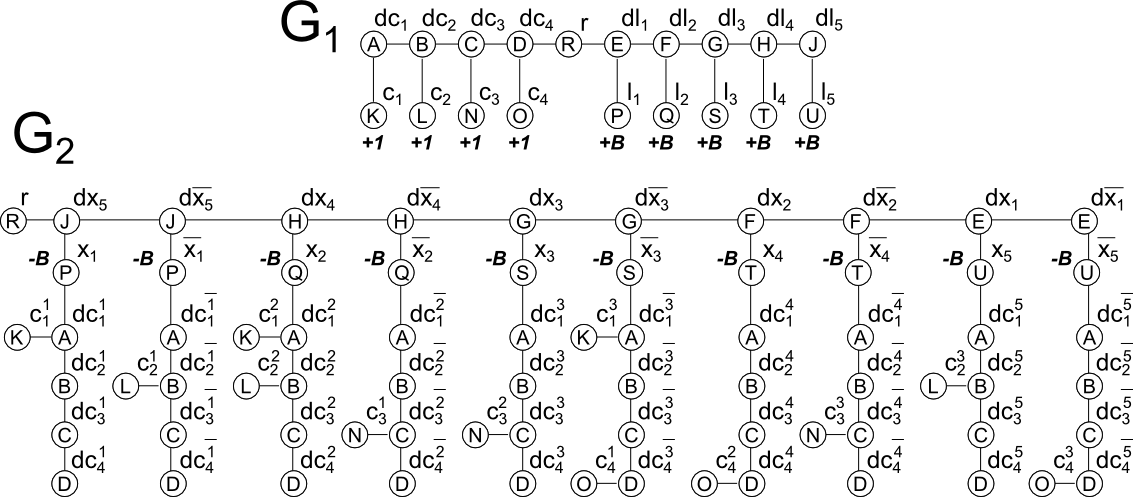
\includegraphics[width=\textwidth]{apx_bt-cater}
    	 	 \caption[Illustration of the construction of $G_1$, $G_2$, and $M$, given $C_q$ (1)]{Illustration of the construction of $G_1$, $G_2$, and $M$, given $C_q = \{(x_1 \vee x_2 \vee \neg{}x_3), (\neg{}x_1 \vee x_2 \vee x_5), (\neg{}x_2 \vee x_3 \vee \neg{}x_4), (\neg{}x_3 \vee x_4 \vee \neg{}x_5)\}$. For readability, the mapping $M$ is not drawn but represented as labels located on the nodes: any pair of nodes (one in $G_1$ and one in $G_2$) of similar inner label are mapped in $M$.}
			\label{fig:bt-cater}
		\end{figure}

		Let us prove that this construction is indeed an L-reduction from \msat{}. More precisely, we prove the following property.
		\begin{lemma}
		There exists an assignment of $V_n$ satisfying at least $m$ clauses of $C_q$ if and only if there exists a solution to \mwccs{} of weight at least $m$.
		\end{lemma}

		\begin{proof}
		{\parindent0pt
		$\boxed{\Rightarrow}$ Given} an assignment $\mathcal{A}$ of $V_n$ satisfying $m$ clauses of $C_q$, we construct a solution to \mwccs{} of weight $m$ as follows.

		\begin{align*}
		\text{Let }V_1^*= &V_1 \setminus \{c_j ~\vert~ c_j\ \text{is not satisfied by the assignment}\}\text{ and}\\
		V_2^*= & \{r\} ~\cup \\
		& \{c^k_j ~\vert~ c_j \text{is satisfied by its } k\text{-th literal}\}  ~ \cup \\
		& \{x_i, dc^i_j ~\vert~ x_i=1, 1 \leq j \leq q\} ~\cup \\
		& \{\overline{x_i}, dc^{\overline{i}}_j ~\vert~ x_i=0, 1 \leq j \leq q\} ~\cup \\
		& \{dx_i,d\overline{x_i} ~\vert~ 1 \leq i \leq n\}.
		\end{align*}

		By construction, $G_1[V_1^*]$ is connected since all the vertices of the spine of the caterpillar have been kept. Moreover, $G_1[V_1^*]$ contributes $B \times n+m$ to the overall weight of the solution, that is $B$ for each of the $l_i$ and $+1$ for each satisfied clause.
		By construction, all the sub-trees rooted at $x_i$ (resp. $\overline{x_i}$) are kept in $G_2[V_2^*]$ if $x_i=1$ (resp. $x_i=0$) in $\mathcal{A}$. Moreover, all the dummy nodes for literals ($dx_i$ and $d\overline{x_i}$) and the root $r$ have been kept. Thus, $G_2[V_2^*]$ is also connected.
		Furthermore, $G_2[V_2^*]$ contributes to $-B\times n$ to the overall weight of the solution since exactly one of each variable node ($x_i$ and $\overline{x_i}$) has been kept. 
		One can easily check that any node of $V_1^*$ has a mapping counterpart in $V_2^*$. The overall solution is valid and of total weight $m$.

		\vspace*{1em}
		{\parindent0pt
		$\boxed{\Leftarrow}$ Given any solution $\{V_1^*,V_2^*\}$ to \mwccs{} of weight $m$, we construct a solution to the \msat{} problem satisfying at least $m$ clauses as follows.
		}

 	 	 First, note that we can assume that any such solution to \mwccs{} is \textit{canonical}, meaning that $V_2^*$ does not contain both vertices $x_i$ and $\overline{x_i}$ for all $1\leq i\leq n$. Indeed, by contradiction, suppose there exists a solution such that $\{x_i,\overline{x_i}\}\subseteq V_2^*$ for a given $1\leq i \leq n$. Then, $\{x_i,\overline{x_i}\}$ in $G_2$ induce a negative weight of $-2B$. This negative contribution can at most be compensated by the weight of the corresponding literal node in $G_1$ ($w_1(l_i)=B$) and at most $B$ clause nodes in $G_1$ ($B \geq \sum w_1(c_j)$ where $x_i\in c_j\ or\ \overline{x_i}\in c_j$) since every literal occurs in at most $B$ clauses in $C_q$. Therefore, such local configuration does not provide any positive contribution to the solution and can be transformed into a better solution by removing one of the sub-trees rooted in $\{x_i,\overline{x_i}\}$. We will consider hereafter that $m$ is the weight of the resulting canonical solution. We further assume that $m>1$ since otherwise we can build a trivial assignment $\mathcal{A}=\{c^1_1=1\}$ of $V_n$ that is satisfying at least one clause of $C_q$.

		Let $\mathcal{A}$ be an assignment of $V_n$ such that for all $1\leq i\leq n$ if $x_i\in V_2^*$ then $x_i=1$ and $x_i=0$ otherwise. Note that, since our solution is canonical, each literal has been assigned a single boolean value in $\mathcal{A}$. Let us now prove that this assignment satisfies at least $m$ clauses of $C_q$.

		First, note that since our solution is canonical and we require any node of $V_1^*$ to have a mapping counterpart in $V_2^*$, this implies that if $l_i\in V_1^*$ then its contribution (that is $w_1(l_i)=B$) is cancelled by the negative contribution of either $x_i$ or $\overline{x_i}$ in $V_2^*$ (that is $w_2(x_i)=w_2(\overline{x_i})=-B$). Therefore, the weight $m$ of the solution can only be realized by $m$ clause nodes of $G_1$, say $\mathcal{C}_1\subseteq V_1^*$ -- since $w_1(c_j)=1$ for all $1\leq j \leq q$.

		As already stated, to be part of the solution any node in $V_1^*$ has a mapping counterpart in $V_2^*$. Thus, for each node in $\mathcal{C}_1$, there should be a node of $\mathcal{C}_2 \subseteq \{c_j^k ~\vert~ 1\leq j \leq q, 1\leq k\leq 3\}$ in $V_2^*$. More precisely, by construction, any node $c_j$ in $V_1$ has exactly three mapping counterparts in $V_2$ (that is $\{c_j^k ~\vert~ 1\leq k \leq 3\}$) and for each $c_j\in \mathcal{C}_1$ at least one of these mapping counterparts has to belong to $\mathcal{C}_2$.

		Finally, since both $G_1[V_1^*]$ and $G_2[V_2^*]$ have to be connected, each node in $\mathcal{C}_2$, say $c_j^k$, should be connected by a path to a node $x_i$ or $\overline{x_i}$, say $x_i$, for some $1\leq i \leq n$, in $G_2[V_2^*]$. By construction, this is the case if $x_i$ is the $k$-th literal of the clause $c_j$ for some $1\leq k \leq 3$. Thus, $\mathcal{A}$ is an assignment that satisfies any clause $c_j$ such that the clause node $c_j$ belongs to $V_1^*$. As already stated $|\mathcal{C}_1|=m$.
		\end{proof}

		The above reduction linearly preserves the approximation since the weights of optimal solutions of the problems correspond and there exists an assignment of $V_n$ satisfying at least $m$ clauses of $C_q$ if and only if there exists a solution to \mwccs{} of weight at least $m$. Hence, given an approximation to \mwccs{}, one can derive an algorithm for \msat{} with the same approximation ratio. Since \msat{}, $B\geq 3$, is APX-hard \parencite{papadimitriou1991optimization} and \msat{} for $B=6$ is not approximable within factor $1.0014$ \parencite{berman1999some}, so is \mwccs{}, which proves \Cref{prop:apx-bt-cater}.

		Let us now prove a similar result for \mwccs{} problem when the mapping is a bijective function.


		\subsection{Bijective relationship function, tree, and graph}
		\label{subsec:apx-t-graph}

		\begin{proposition}\label{prop:apx-t-graph}
  	  	  The \mwccs{} problem for a graph and a tree is APX-hard and not approximable within factor $1.0014$ even when the mapping is a bijective function.% and a complete conservation (i.e. $\alpha = 1$) is required.
		\end{proposition}

		Given any instance $(C_q,V_n)$ of \msat{}, we build a graph $G_1=(V_1,E_1)$ with weight function $w_1$, a tree $G_2=(V_2,E_2)$ with weight function $w_2$ and a mapping $M$ as follows. The graph $G_1$ has the vertex set $V_1=\{r, l_i, x_i, \overline{x_i}, c_j,$ $ c^k_j ~\vert~ 1\leq i\leq n, 1\leq j \leq q, 1\leq k \leq 3\}$ and the edge set defined by the following equation.
		\begin{align*}
		E_1= & \{(l_i,x_i), (l_i,\overline{x_i}), (r,x_i), (r,\overline{x_i}) ~\vert~ 1\leq i\leq n\} ~\cup  \\
 	 	 & \{(c_j,c_j^k), (r,c_j^k)  ~\vert~ 1\leq k \leq 3, 1\leq j \leq q\}.
		\end{align*}

		The weight function $w_1$ is defined as follows: for all $1\leq k \leq 3$, $1\leq i\leq n$ and $1\leq j \leq q$, $w_1(l_i)=B$, $w_1(c_j)=1$ and $w_1(r)=w_1(c_j^k)=w_1(x_i)=w_1(\overline{x_i})=0$.

		Roughly, in $G_1$ there is a node for each clause (denoted by $c_j$), for each of the three literals of each clause (denoted by $c_j^k$), for each literal (denoted by $l_i$) and for each valuation of each literal (denoted by $x_i$, $\overline{x_i}$). Clause nodes and literal nodes are separated by a central node $r$.

		The tree $G_2$ is defined as follows. The vertex set is $V_2=V_1$, the edge set is given by the following equation:
		\begin{align*}
		E_2= & \{(l_i,r), (c_j,r), (x_i,r), (\overline{x_i},r) ~\vert~ 1\leq i\leq n, 1\leq j \leq q\} ~\cup \\
		& \{(c^k_j,x_i) ~\vert~ x_i \text{ is the  } k\text{-th literal of clause } c_j\} ~\cup\\
		& \{(c^k_j,\overline{x_i}) ~\vert~ \overline{x_i} \text{ is the } k\text{-th literal of clause } c_j\}.
		\end{align*}

		The weight function $w_2$ is defined as follows: for all $1\leq k \leq 3$, $1\leq i\leq n$ and $1\leq j \leq q$, $w_2(x_i)=w_2(\overline{x_i})=-B$, $w_2(r)=w_2(c_j^k)=w_2(l_i)=w_2(c_j)=0$.


		Roughly, in $G_2$ all the nodes except the ones in $\{c_j^k~\vert~ 1\leq j \leq q, 1\leq k\leq 3\}$ form a star centered in node $r$. The nodes representing the literal of the clause (that is $c_j^k$) are connected to their corresponding variable nodes (that is $x_i$ or $\overline{x_i}$).

		Finally, the mapping $M$ is a bijective function from $V_1$ to $V_2$ defined as the identity (that is each node in $V_1$ is mapped to the node of similar label in $V_2$).


		\begin{figure}[ht]
    	 	 
    	 	 \centering
    	 	 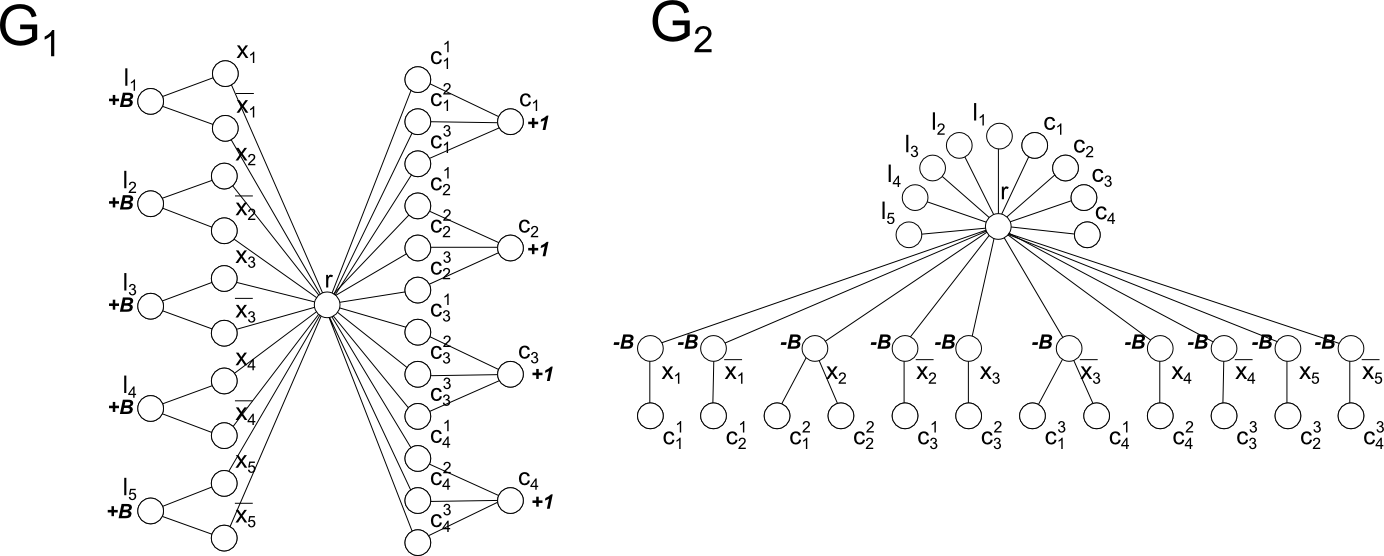
\includegraphics[width=\textwidth]{apx_g-tree}
    	 	 \caption[Illustration of the construction of $G_1$, $G_2$, and $M$, given $C_q$ (2)]{Illustration of the construction of $G_1$, $G_2$, and $M$, given $C_q = \{(x_1 \vee x_2 \vee \neg{}x_3), (\neg{}x_1 \vee x_2 \vee x_5), (\neg{}x_2 \vee x_3 \vee \neg{}x_4), (\neg{}x_3 \vee x_4 \vee \neg{}x_5)\}$. For readability, the mapping $M$ is not drawn but deduced from the labels of the nodes; any pair of nodes (one in $G_1$ and one in $G_2$) of similar label are mapped in $M$.}\label{fig:g-tree}
    	 	 \end{figure}
   		
		Let us prove that this construction is indeed an L-reduction from \msat{}. More precisely, we prove the following property.

		\begin{lemma}
 	 	 There exists an assignment of $V_n$ satisfying at least $m$ clauses of $C_q$ if and only if there exists a solution (not necessarily optimal) to \mwccs{} of weight at least $m$.
		\end{lemma}

		\begin{proof}

		{\parindent0pt
		$\boxed\Rightarrow$} Given an assignment $\mathcal{A}$ of $V_n$ satisfying $m$ clauses of $C_q$, we construct a solution to \mwccs{} of weight $m$ as follows.

		Let $V_1^*=V_2^*=\{c_j~\vert~ c_j \text{ is satisfied by } \mathcal{A}\} \cup \{c^k_j~\vert~ c^k_j \text{ is satisfying } c_j \text{ by } \mathcal{A}\}\cup\{x_i~\vert~ x_i=1\}\cup\{\overline{x_i}~\vert~ x_i=0\}\cup \{r,l_i~\vert~ 1\leq i\leq n\}$. 

		By construction, $G_1[V_1^*]$ and $G_2[V_2^*]$ are connected. Moreover, $G_1[V_1^*]$ contributes $B\times n+m$ to the overall weight of the solution, that is $B$ for each of the $l_i$ and $+1$ for each satisfied clause, while $G_2[V_2^*]$ contributes $-B\times n$ to the overall weight of the solution since exactly one of each variable node ($i.e.$, $x_i$ and $\overline{x_i}$) has been kept. The overall solution is valid and of total weight $m$.

		\vspace*{1em}
		{\parindent0pt
		$\boxed{\Leftarrow}$} Given any solution $V^*\subseteq V_1$ to \mwccs{} of weight $m$, we construct a solution to the \msat{} problem satisfying at least $m$ clauses as follows.

		First, note that, as in the previous construction, we can assume that any such solution to \mwccs{} is \textit{canonical} meaning that $V^*$ does not contain both vertices $x_i$ and $\overline{x_i}$ for any $1\leq i\leq n$.

		Let $\mathcal{A}$ be an assignment of $V_n$ such that for all $1\leq i\leq n$, if $x_i\in V^*$ then $x_i=1$ and $x_i=0$ otherwise. Note that, since our solution is canonical, each literal has been assigned a single boolean value in $\mathcal{A}$. Let us now prove that this assignment satisfies at least $m$ clauses of $C_q$.

		First, note that since our solution is canonical, as in the previous construction, the weight $m$ of the solution can only be induced by $m$ clause nodes of $G_1$, say $\mathcal{C}_1\subseteq V^*$.

		Since both $G_1[V^*]$ and $G_2[V^*]$ have to be connected, any solution with $m>1$ will include node $r$ in $V^*$. Thus, for each node $c_j\in\mathcal{C}_1$ there should be a node of $\{c_j^k ~\vert~ 1\leq k\leq 3\}$ in $G_1[V^*]$ to connect $c_j$ to $r$. In $G_2[V^*]$, in order for nodes $r$ and $c_j^k$ to be connected, the corresponding literal node (that is $x_i$ or $\overline{x_i}$), say $x_i$ -- has to be kept in $V^*$. By construction, this is the case if $x_i$ is the $k$-th literal of clause $c_j$. Thus, $\mathcal{A}$ is an assignment that satisfies any clause $c_j$ such that the clause node $c_j$ belongs to $V^*$. As already stated $|\mathcal{C}_1|=m$.
		\end{proof}

		The above reduction linearly preserves the approximation and proves \Cref{prop:apx-t-graph}.

%		\subsubsection{Binary tree and graph}
%		\label{subsubsec:binary-tree}
%
%		XXX refaire si temps le permet XXX

	\section{Polynomial-time cases for the \mwccs{} problem}
	\label{sec:poly}

%%%		\subsection{Two bounded-degree trees and a bijective mapping}
%%%		\label{subsec:tree1o1}
%%%
%%%			We have proved in \cref{subsec:apx-bt-cater} that for instances with two binary trees, and an injective mapping function, the problem is APX-hard.
%%%			We will now consider the case of two bounded-degree trees, $T_1 = (V_1, E_1)$ and $T_2 = (V_2, E_2)$, with a bijective relationship, or mapping function, $V_1\,M\,V_2$. Without loss of generality, lets now suppose that their respective degrees are $d_{T_1} = d_{T_2} = d$, and that $\norm{V_1} = \norm{V_2} = n$.
%%%
%%%%			The standard algorithms for \mwcs{} and its variants\footnote{Mainly cardinality-constrained, budget-constrained, and ratio-bounded, with a pseudo-polynomial algorithm for all of them exposed in the next chapter.} use bottom-up, usually dynamic-programming, approaches.
%%%%			Given an unrooted tree $T$, root $T$ in one of its node to direct the edges.
%%%%			Then, compute recursively the maximum weight of the subtrees that unconditionally includes their root.
%%%
%%%%			It would be a good characteristic of our algorithm to advance in a similar fashion, recursively solving subproblems, and progressing in both trees in locked step.
%%%			Since $\alpha=1$, a node can only be selected if its counterpart is also selected.
%%%			However, note that a node in one of the trees %\footnote{With any arbitrary node as its root.}
%%%			can have its counterpart at a completely different depth in the other tree %\footnote{Also with any arbitrary node as its root.}
%%%			 (see \cref{fig:childReqParent}).
%%%			Consequently, adding a child node might require the addition of a parent by mutual requirement between the two trees and the mapping function (see \cref{fig:childReqParent}).
%%%			This exhibit the main difficulty with this problem: the non-isomorphic mapping function makes it impossible to use the usual local dynamic programming scheme to solve the \mwcs{} problem and its variants on trees.
%%%
%%%			\begin{figure}[ht]
%%%				\centering
%%%            \begin{tikzpicture}[level/.style={sibling distance=9em/#1},
%%%              every node/.style = {shape=circle, draw, align=center, minimum size=2.3em}]]
%%%              \node {R}
%%%                child { node {A}
%%%                  child { node {\phantom{N}} }
%%%                  child { node {\phantom{N}} }
%%%                }
%%%                child { node {C}
%%%                  child { node {\phantom{N}} }
%%%                  child { node {B} }
%%%                };
%%%            \end{tikzpicture}
%%%            \qquad
%%%            \begin{tikzpicture}[level/.style={sibling distance=9em/#1},
%%%              every node/.style = {shape=circle, draw, align=center, minimum size=2.3em}]]
%%%              \node {r}
%%%                child { node {b}
%%%                  child { node {a} }
%%%                  child { node {c} }
%%%                }
%%%                child { node {\phantom{N}}
%%%                  child { node {\phantom{N}} }
%%%                  child { node {\phantom{N}} }
%%%                };
%%%            \end{tikzpicture}
%%%
%%%%				\includegraphics[width=\textwidth,height=0.3\textwidth]{childReqParent.png}
%%%				\caption[Nodes labeled with the same letter are counterpart of one another]{Nodes labeled with the same letter are counterpart of one another.
%%%				When starting from an empty solution\protect\footnotemark, the inclusion of node $A$ requires only the inclusion of $a$. However when starting from the root nodes, the inclusion of node $A$ requires the inclusion of node $a$, which recursively requires the inclusions of $b$, $B$, $C$, and $c$.
%%%				A local dynamic programming approach is impossible since the context is important.}
%%%				\label{fig:childReqParent}
%%%			\end{figure}
%%%
%%%			In this section, we introduce a \emph{functional dynamic programming} approach for this setup that solve the \mwccs{} problem in polynomial time parameterized on the degree of the trees. A functional dynamic programming approach is a \emph{top-down} dynamic programming technique, that is recursive and using subproblem overlaps, that uses a \emph{memoization} scheme to store intermediate results instead of the usual tabular approach.
%%%
%%%			Our algorithm is composed of two main operations.
%%%			$\text{ComputeDecisionTree}$ is the main functionnal dynamic programming procedure and finds the optimal solution to the problem given two trees and a root for one of them.
%%%			$\text{ComputeDecisionTree}$ calls upon $\text{ConstructRequiredSet}$ to maintain the connectivity and matching constraints of the candidate solution.
%%%			%Now the complete operations might seem unnecessarily complex for now, but will become self-explanatory in the end.
%%%
%%%			\footnotetext{As is the case with regular dynamic programming, which depend only on local subproblems.}
%%%
%%%			\paragraph{$\text{ConstructRequiredSet}$:}
%%%			Informally, $\text{ConstructRequiredSet}$ takes as input all the nodes that have been included up intil now, from both $T_1$ and $T_2$, and add into those sets all nodes that are required to be added if $u$ is included to keep 1) connectivity and 2) perfect matching (see \cref{fig:childReqParent}).
%%%
%%%			Adding a node $u \in V_1$ from $T_1$ to a candidate solution\footnote{At least one of the neighbors of $u$ is in the candidate solution, or the candidate solution is empty. That is, its addition leaves the candidate solution connected.} requires the unconditional inclusion of its counterpart $v \in V_2$ from $T_2$ to the candidate solution.
%%%			In turn, the addition of $v$ requires the addition of all nodes from $T_2$ that are necessary for the candidate solution to remain connected: the (possibly empty) shortest path $v_0 v_1 \ldots v_i$ between $v$ and, if one exists, its closest node from $T_2$ already in the solution.
%%%			Recursively, this requires the addition of all counterparts of the nodes $v_0$, $v_1$, $\ldots$, $v_i$ to the candidate solution, and the nodes required for the candidate solution to remain connected.
%%%			This recursion continues until no more nodes are required to be included to conserve connectivity.
%%%
%%%			It is formally defined as follows.
%%%			Given two sets $S_1 \subseteq V_1$ and $S_2 \subseteq V_2$ of nodes already selected, and a node $u \in V_1 \setminus S_1$ such that $u$ is a neighbor of a node in $S_1$ ($v \in V_2$ its counterpart).
%%%			We define a double recursion procedure over $V_1$ and $V_2$.
%%%			Add $u$ to $S_1$; then, find the shortest path from its counterpart $v$ to any node of $S_2$.
%%%			Add all nodes that pertain to this shortest path to $S_2$ (including $v$), and recursively find all shortest paths from their counterparts to the nodes of $S_1$.
%%%			%Note that since the graphs are trees, the order which is used to call the procedure on all these nodes can be arbitrary.
%%%			Continue until no more nodes need to be added.
%%%
%%%			\begin{proposition}\label{prop:constructFuncConnected}
%%%				The induced graphs $T_1[S_1]$ and $T_2[S_2]$ obtained as results of $\text{ConstructRequiredSet}$ are connected.
%%%			\end{proposition}
%%%			\begin{proof}
%%%				Indeed, since we recursively add nodes with their shortest path to already selected nodes, there exists a path connecting every pairs of nodes of $S_1$ and of $S_2$.
%%%			\end{proof}
%%%
%%%			\begin{proposition}\label{prop:constructFuncQuadratic}
%%%				$\text{ConstructRequiredSet}$ is a quadratic operation in the worst case.
%%%			\end{proposition}
%%%			\begin{proof}
%%%				The shortest path toward a set of nodes in a tree is equivalent to the minimum sum subsequence problem and can be solved in linear time using a dynamic programming approach.
%%%				We recursively add up to $O(n)$ nodes (all).
%%%				Hence the resulting complexity.
%%%			\end{proof}
%%%
%%%			\paragraph{$\text{ComputeDecisionTree}$:}
%%%			The main procedure, $\text{ComputeDecisionTree}$,  is a recursive decision tree traversal of $T_1$ that uses the $\text{ConstructRequiredSet}$ operation.
%%%%			This recursive procedure, $\text{ComputeDecisionTree}$ is formally defined as follows.
%%%%			Given two sets $S^u_1$ and $S^u_2$ of connected nodes in $V_1$ and $V_2$ respectively, and a node $u$: the last selected node in the decision tree.
%%%%			Lets define $u^i$ the $i$-th children of $u$, and $C_u = \bigcup\limits_i{u^i}$ the set of these children. %, and $C = C_u \setminus S_1$ the children of $u$ that where not added to $S_1$ in any of the previous decisions.
%%%%			%If all children of $u$ have been recursively added at the previous step ($C = \emptyset$), end this branch of the decision tree.
%%%%			%If $u$ has not children ($C = \emptyset$), end this branch of the decision tree.
%%%%			For all nodes $u^i \in C_u$, if any:
%%%%			\begin{enumerate}
%%%%				\item call the $\text{ConstructRequiredSet}$ procedure with $S^u_1$, $S^u_2$, and $u^i$, which will return $S^{u_i}_1$ and $S^{u_i}_2$, and
%%%%				\item recursively expend the decision tree by calling $\text{ComputeDecisionTree}$ with $S^{u_i}_1$, $S^{u_i}_2$, and $u^i$.
%%%%			\end{enumerate}
%%%%			We then compute a score $s(S_1, S_2, u)$ for this node (defined by the selection of $u$ in the decision tree) as follows.
%%%			It is formally defined as follows.
%%%			Given $T_1$, $T_2$, and a node $u \in V_1$, this function returns the set $S^u_1$ and $S^u_2$: the best selection of nodes, respectively from $T_1$ and $T_2$, when optimizing in the subtree rooted in $u$ and which includes $u$.
%%%			Note that $S^u_1$ might contain nodes that are parents to $u$, as a requirement for the matching and connectivity constraints.
%%%			Lets define $u_i$ the $i$-th children of $u$, and $C^u = \bigcup\limits_i{\{u_i\}}$ the set of these children. %, and $C = C_u \setminus S_1$ the children of $u$ that where not added to $S_1$ in any of the previous decisions.
%%%			%If all children of $u$ have been recursively added at the previous step ($C = \emptyset$), end this branch of the decision tree.
%%%			%If $u$ has not children ($C = \emptyset$), end this branch of the decision tree.
%%%			For all nodes $u_i \in C^u$, if any:
%%%			\begin{enumerate}
%%%				\item recursively call $\text{ComputeDecisionTree}$ with $u_i$, which will return the sets $S^{u_i}_1$ and $S^{u_i}_2$, then
%%%				\item call the $\text{ConstructRequiredSet}$ procedure with $S^{u_i}_1$, $S^{u_i}_2$, and $u$, which will return $\accentset{\circ}{S^{u_i}_1}$ and $\accentset{\circ}{S^{u_i}_2}$.
%%%			\end{enumerate} 
%%%			Then compute a score $s(u)$, which correspond to the optimal combination of children such that their inclusion maximizes the local sum of weights.
%%%			This score only consider the subtree rooted in $u$ and including $u$ in a typical dynamic programming approach.
%%%
%%%			Formally, the computation of this score is as follows.
%%%			For notation sake, lets define $\mathcal{P}^u = \mathcal{P}\left({C^u}\right)$: the \emph{power set} containing all the combinations of children of $u$; and $\mathcal{P}^u_k$ the $k$-th element of this set.
%%%			Lets also define $S^{\mathcal{P}^u_k} = \bigcup\limits_{u^i \in \mathcal{P}^u_k}{\accentset{\circ}{S^{u_i}_1} \cup \accentset{\circ}{S^{u_i}_2}}$: the union of the optimal nodes in the $k$-th combination of children\footnote{Note that in general, this union is certainly not optimal. Unless there are multiple optimal solutions, only one combination of the children maximizes the score, and possibly the empty one.}, including $u$.
%%%			To simplicity notation, we further define $S^{\mathcal{P}^u_0}$, with the $0$-th combination being the usual empty set\footnote{Here of children.}, as the set $\{u, v\}$: if no children are selected, only the current node and its counterpart are part of the solution, which is a connected and matched solution by definition.
%%%			Finally, we have:
%%%%			\[
%%%%				w(S^{d_i}) = w(n_i) + \max\left(0, w\left(S^{{\langle r\rangle}_{d_i}}\right), w\left(S^{{\langle r\rangle}_{d_i}}\right), w\left(S^{{\langle l\rangle}_{d_i}} \cup S^{{\langle r\rangle}_{d_i}}\right)\right)
%%%%			\]
%%%%			\[
%%%%			s(u) = w(u) + \max\left(\begin{array}{c}
%%%%				0,\\
%%%%				w\left(S^{{\langle \text{left}\rangle}_{d_i}}\right),\\
%%%%				w\left(S^{{\langle \text{right}\rangle}_{d_i}}\right),\\
%%%%				w\left(S^{{\langle \text{left}\rangle}_{d_i}} \cup S^{{\langle \text{right}\rangle}_{d_i}}\right)
%%%%			\end{array}\right)
%%%%			\]
%%%%			\begin{align*}
%%%%				s(u)
%%%%					& = \sum\limits_{n \in S^u}{w(n)} + \max\limits_{k}{\left(0, \sum\limits_{n \in S^{\mathcal{P}^u_k} \setminus S^u}{w(n)}\right)} \\
%%%%					& = \max\limits_{k}{\left(\sum\limits_{n \in S^u}{w(n)}, \sum\limits_{n \in S^{\mathcal{P}^u_k}}{w(n)}\right)}
%%%%			\end{align*}
%%%			\[
%%%				s(u) = \max\limits_{k}{\sum\limits_{n \in S^{\mathcal{P}^u_k}}{w\left(n\right)}}
%%%			\]
%%%
%%%			Computing the optimal combination of children, required for the $\max$ function, is not an easy problem.
%%%			It looks similar to the \textsc{weighted maximum coverage} problem \parencite{hochbaum1996approximation}, relaxed both with possibly negative weights, and with unconstrained number of sets.
%%%			It also looks quite similar to the \textsc{set-union knapsack} problem \parencite{goldschmidt1994note}, but again with real-valued weights and without budget constraint.
%%%			Both are sensibly related and difficult, NP-hard problems~\parencites{hochbaum1996approximation,cohen2008generalized}.
%%%			However, since we are working with bounded-degree trees, the number of combinations remains (parameterized-)constant. The overall algorithm is thus in FPT (Fixed-Parameter Tractable), see \cref{prop:decisionTreeComplexity} for proof.
%%%
%%%			\begin{proposition}
%%%				$\text{ComputeDecisionTree}$ is a parameterized complexity algorithm which requires at most $O(2^d n^2 + n^3)$ steps for $d$-ary trees.
%%%				\label{prop:decisionTreeComplexity}
%%%			\end{proposition}
%%%			\begin{proof}
%%%				The recursion tree closely follows the topology of $T_1$, and contains at most $O(n)$ calls.
%%%				At each step we use the $\text{ConstructRequiredSet}$ procedure, which is a quadratic time operation.
%%%				We also compute the score, which itself requires to compute a set union operation for each combination of children.
%%%				There are at worst $O(2^d)$ combination of children (the cardinality of the power set), and set union is at worst an $O(n)$ operation with a bitvector representation of the sets.
%%%				Hence the resulting number of steps.
%%%			\end{proof}
%%%
%%%%			\paragraph{}
%%%%			Overall, note that this procedure construct increasingly inclusive set of required nodes $S_1$ and $S_2$.
%%%%			This is expected, since recursive calls can only add nodes to the solution in order to maintain the two connectivity and matching contraints after each decision.
%%%%			However, it effectively defines an environment into which the recursive $\text{ComputeDecisionTree}$ operate, implicitly defined by the initial node and the set of choices made up until the current node.
%%%%
%%%%			
%%%%
%%%%			\begin{figure}[ht]
%%%%				\centering
%%%%				\includegraphics[width=\textwidth,height=0.3\textwidth]{DecisionTreeWithScores.png}
%%%%				\label{fig:foo}
%%%%			\end{figure}
%%%%
%%%%			We thus need to iterate this decision tree procedure for all pairs $u,v \in V_1\times V_2$.
%%%
%%%			\begin{proposition}
%%%				One of the recursive calls of $\text{ComputeDecisionTree}$ contains the optimal solution to the global problem.
%%%			\end{proposition}
%%%			\begin{proof}
%%%				Even though two subtrees could actually have the exact same solution, since parent nodes can be included for matching and connectivity constraint reasons, it should be clear from the standard tree traversal that the whole tree $T_1$ is considered and that all its subtrees (that respect the constraints) are evaluated.
%%%				To see that the optimal solution found by this procedure, in $T_1$, is also the optimal in regard to $T_2$, note that any given subtree of $T_1$, that is valid under the constraints, have one and only one counterpart subtree in $T_2$.
%%%				Indeed, since the matching is a bipartite function, each node have one and only one counterpart; any subtree of size $m$ in $T_1$ have one and only one counterpart subtree of size $m$ in $T_2$, the one that contains all counterpart nodes.
%%%				Finally, since all possible subtrees of $T_1$ (that respect the constraints) are considered, it must be that all possible subtrees of $T_2$ are also considered by this procedure.
%%%			\end{proof}
%%%
%%%			The optimum is in the recursive call with the highest total score, the optimal objective, and the optimal solution is the corresponding set of nodes $S^u$.
%%%
%%%%			\begin{proposition}\label{prop:totalComplex}
%%%%				The overall algorithm to compute the optimal solution is an $O(n^3)$ running time algorithm.
%%%%			\end{proposition}
%%%%			\begin{proof}
%%%%				Indeed, since the nodes are on a one to one mapping, there exists exactly $n = \norm{V_1} = \norm{V_2}$ pairs of nodes $u,v \in V_1\times V_2$.
%%%%				For each such pair we call $\text{ComputeDecisionTree}$ which is an $O(n^2)$ operation.
%%%%
%%%%				In the end, the optimal solution is in one of the $O(n^3)$ decision tree nodes.
%%%%
%%%%				Hence the total running time.
%%%%			\end{proof}
%%%
		\subsection{Polynomial-time scheme for some inputs}
		\label{subsec:enumerable}

			Notice that in the previous sections the conservation constraint $\alpha$ for the solution, that defines which fraction of nodes has to be kept, has been strict; that is $\alpha = 1$.
			Here we consider where $\alpha \in [0,1]$.
			In addition, we further relax the constraint on the mapping function, which can be any partial injective function.
			That is, any element of $V_1$ can have at most one image in $V_2$ (the elements of $V_2$ can have 0, 1, or more antecedents).
			Finally, we suppose that there is a polynomial number of connected induced subgraphs of $G_1$.

			We consider as many candidate solutions as there are connected subgraphs of $G_1$, and for each one of them we try to find the best corresponding subgraph in $G_2$.
			The best corresponding subgraph in $G_2$ is the subgraph that maximizes the total weight of the candidate solution and such that at least an $\alpha$-fraction of the nodes of $G_1$ and $G_2$ in the solution are $M$-related.
			For a given subgraph of $G_1$, the sum of the weights of its nodes is fixed.
			Hence maximizing the total weight of the candidate solution is equivalent to finding the optimal solution in $G_2$ where the $\alpha$-fraction constraint holds.

			To solve this problem, we introduce a new problem, the \textsc{ratio-bounded maximum-weight connected subgraph} (\rbmwcs) problem.
			Informally, it consists in a variant of the \mwcs{} problem where an additional contribution function is associated to each node and where an additional ratio constraint is introduced, not unlike the \emph{budget-constrained} variant of the \mwcs{} problem.
			This new problem is formally defined in \cref{sec:rbmwcs}.

			The reduction to this new subproblem is as follows.
			The contribution function needs to \emph{encode} the relationship function between the nodes of both $G_1$ and $G_2$.
			To do so, and since we fixed a partial solution to the problem in the form of the subgraph of $G_1$, we note for each node of $G_2$ its number of inverse images in $G'_1$ plus one if and only if at least one exists, zero otherwise.
			The reason we need to make the distinction between the two cases is that when there is no counterpart in $G_1$, selecting a node in the optimal solution in $G_2$ will not increase the number of mapped node overall.
			However, selecting a node in $G_2$ for which there exists at least one counterpart will increase the number of mapped node by the number of counterpart, plus one for the selected node itself.

			Formally, given a connected subgraph $G'_1=(V'_1,E'_1)$ of $G_1$, we define the corresponding $G_2$ \emph{antecedent function} $a\colon V_2 \to \mN$ to be $a(v)=\card{\Set{v,u}{M(u,v), u\in V'_1}}$.
			The \emph{contribution function} $c\colon V_2 \to \mN$ is defined as follows:
			$$c(v)=\begin{cases}a(v) + 1 &\mbox{if }a(v) > 0\mbox{,} \\
		                       0        &\mbox{otherwise.}
		          \end{cases}$$

			Given $G_2=(V_2,E_2)$, its weight-function $w_2$ and its contribution function $c$, the problem now corresponds to the discovery of the connected subgraph of maximum weight such that:
			\begin{align*}
				\sum_{v \in V^*_2}{c(v)}                           &\geq \alpha\times\left(\norm{V'_1} + \norm{V^*_2}\right) \\
				\sum_{v \in V^*_2}{c(v)} - \alpha\times\norm{V'_1} &\geq \alpha\times\norm{V^*_2}
			\end{align*}
			Where $\alpha\times\norm{V_1'}$ is constant.

			Finally, given the optimal score of all candidate solutions, for which there are one for each subgraphs $G'_1$, the optimal solution to the \mwccs{} problem is the one candidate solution among them which has the best score.

			Clearly, constructing a contribution function for $G_2$ given a subgraph $G'_1$ is a linear time operation.
			Choosing the best candidate solution is as time consuming as enumerating all subgraphs of $G_1$, which is a polynomial time operation in this context.
			The complexity of this algorithm hence depends on the difficulty to solve the \rbmwcs{} subproblem.

			\Cref{sec:rbmwcs} provides an analysis of this problem with a more general contribution function.
%			It provides pseudo-polynomial scheme for all classes of input graphs up to bounded treewidth.
			It provides polynomial scheme for $d$-ary trees and an optimized algorithm for paths.
%			However, when the contribution function is enumerable with a polynomial upper bound, and such is the case by construction here, the scheme actually becomes a polynomial-time algorithm.
%			Thus, there exists a polynomial-time algorithm to solve \mwccs{} when one of the graph if polynomially enumerable, the second is bounded treewidth, and the relationship is a partial injective function, for any $\alpha \in [0, 1]$.
			Thus, there exists a polynomial-time algorithm to solve \mwccs{} when one of the graph if polynomially enumerable, the second is a bounded-degree tree, and the relationship is a partial injective function, for any $\alpha \in [0, 1]$.

	\section{The Ratio-Bounded Maximum-Weight Connected Subgraph problem}
	\label{sec:rbmwcs}

		In this section, we introduce a slightly more general version than required in \cref{subsec:enumerable}\footnote{The contribution function can represent inputs that we don't actually use.}.
		The \textsc{ratio-bounded maximum-weight connected subgraph} (\rbmwcs) problem, is formally defined as follows.

		\textbf{\rbmwcs{}}: Given a node-weighted graph $G = (V, E)$, its node-weighting function $w\colon V \to \mR$, its contribution function $c\colon V \to \mR$, a ratio $\alpha \in [0,1]$ and a constant $C \in \mR$, find a subset $V^* \subseteq V$ such that:
			\begin{enumerate}
				\item the induced graph $G\left[V^*\right]$ is connected, and
				\item the ratio of the sum of contributions plus some constant over the number of nodes in the solution is greater than or equal to $\alpha$, that is:\\
					$\sum\limits_{v \in V^*}{c(v)} + C \geq \alpha\times\card{V^*}$, and
				\item $\sum\limits_{v \in V^*}{w(v)}$ is maximum.
			\end{enumerate}

		\begin{proposition}
			\rbmwcs{} is at least as difficult as \mwcs{}.
		\end{proposition}
		\begin{proof}
			Indeed, when $c(v) = 1,\,\forall v\in V$, the ratio $\sum\limits_{v \in V^*}{c(v)} / \card{V^*} = 1 \geq \alpha$, and the \mwcs{} and \rbmwcs{} problems are equivalent.
		\end{proof}

		Let us show now that it is in PTIME for bounded-degree trees.
		\begin{proposition}
			\rbmwcs{} is solvable in $O(n^{d+2})$ time for $d$-ary trees.
			\label{prop:boundedDegreeTreesRBMWCS}
		\end{proposition}
		\begin{proof}
			Let us consider the \rbmwcs{} problem for a $d$-ary tree.
			We define a dynamic programming strategy with a $O(n^{d+2})$ time complexity.
			This leads to a polynomial algorithm for $d$-ary trees.
			The basic idea is to define a 3-dimensional table $T$ of size $\card{V}\times \sum_{v\in V}c(v) \times \card{V}$ that stores the maximum weight of a subtree rooted in $v$ of size $s$ and of total contribution $tc$.

			Formally, $\forall v\in V,\,0 \leq tc \leq \sum_{v\in V}c(v),\,0 \leq s \leq |V|$, let us note $v_{\langle i\rangle}$ the $i$-th child of $v$, $1 \leq i \leq d$, we have:
			% \[
			%   \begin{array}{rl}
			%   	T[v][0][0]   &= 0 \\
			%     T[v][tc][s]  &= \mathlarger{\max}_{tc_1,\ldots,tc_d,\,\,s_1,\ldots, s_d}\left(w(v) +
			%                         \mathlarger{\sum}_{1 \leq i \leq d}{T[v_{\langle i\rangle}][tc_i][s_i]}
			%                     \right) \\
			%                  & \vphantom{foo} \\
			%     s.t.\quad tc &= c(v) + \mathlarger{\sum}_{1 \leq i \leq d}{tc_i} \\
			%               s  &= 1    + \mathlarger{\sum}_{1 \leq i \leq d}{s_i}
			%   \end{array}
			% \]

			\[
			  \begin{array}{rl}
					T[v][0][0]   &= 0 \\
				  T[v][tc][s]  &= \max\limits_{tc_1,\ldots,tc_d,\,\,s_1,\ldots, s_d}\left(w(v) +
											 \sum\limits_{1 \leq i \leq d}{T[v_{\langle i\rangle}][tc_i][s_i]}
										\right) \\
									& \vphantom{foo} \\
				  s.t.\quad tc &= c(v) + \sum\limits_{1 \leq i \leq d}{tc_i} \\
								s  &= 1    + \sum\limits_{1 \leq i \leq d}{s_i}
				\end{array}
			\]

			The optimal subtree can be reconstructed from the table by finding the entry with the maximal weight and where the contribution ratio is not violated, and backtracking from that entry on the selected $tc_i$'s and $s_i$'s from the $\max$ function.
			Each entry of the table can be computed in $O(n^{d-1})$ (that is, an integer partition of $\card{V}$ into $d$ parts) time, and since $\sum_{v\in V}c(v) \in O(n)$, there are $O(n^3)$ of them, which leads to the overall complexity.
		\end{proof}

		As paths and cycles are trees of degree $1$, using the preceding result leads to an $O(n^3)$ algorithm for these cases. However, one can achieve a better complexity.

		\begin{proposition}
		  \rbmwcs{} is solvable in $O(n^2)$ time for paths and cycles.
		\end{proposition}
		\begin{proof}
			Let us first consider the \rbmwcs{} problem for paths. Leveraging the linearity of the graph structure, we define a dynamic programming strategy with an $O(n^2)$ time complexity.

			The idea is to define two 2-dimensional tables $T_w$ and $T_{tc}$ with $n^2$ entries each and that store respectively, for each pair of indices, the maximum weight and the total contribution, of the corresponding graph. Let us consider a given orientation in the path with the node at the starting end as the reference node, of index 0. Every candidate solution (a subpath) in the path can then be defined as a pair of positions, the first element being the starting position as an index number, the second element being the size of the candidate solution. The main idea being that increasing the indices one by one enables us to update the weights and total contributions incrementally.

			Formally, let us denote the $k$-th node of the graph in the predefined orientation by $n_k$, we have for all $0 \leq i \leq j \leq n$: 
			\[
			  \begin{array}{rl}
				T_w[i][i]    &= 0 \\
				 T_w[i][j]    &= w(n_{i+j-1}) + T_w[i][j-1] \\
				 \vphantom{foobar} \\
				 T_{tc}[i][i] &= 0 \\
				 T_{tc}[i][j] &= c(n_{i+j-1}) + T_{tc}[i][j-1]
			  \end{array}
			\]

			The optimal subpath is defined by the indices of the entry with the maximal weight and where the contribution ratio is not violated ($i.e.$, for any $(i,j)$ s.t. $T_{tc}[i][j]\geq \alpha \cdot j$).
			Each $O(n^2)$ entry of the tables can be computed in constant time, leading to the overall complexity.
			For cycles, the trick consists in taking any linearization of the cycle and merging two copies of the corresponding linearization as the input path.
			This ensures that we will consider any candidate solution ($i.e.$, simple subpath of the cycle).
			The time complexity is preserved.
		\end{proof}


	\section{Related questions and further work}

		In this contribution we provide the first deep complexity analysis of the \mwccs{} problem.
		A fair number of interesting problems and questions still remains.

		First of all, generalizing the problem to more than two graphs is of practical interest.
		We hypothesize that the most general expression of the problem is to have a, possibly empty, mapping function between each graph.
		However, as we have shown throughout this chapter, the mapping function is an important factor for the complexity of the problem.
%%%	It is expected that the FPT algorithm for $d$-ary trees will remain within the parameterized polynomial time category when generalized to $k$ trees and $\frac{k(k+1)}{2}$ bijective mappings, but formal proof remains to be done.
		Since the \mwccs{} problem is APX-hard for two graphs, the hardness results should hold for $k > 2$ graphs.
		However it is unclear whether the polynomial-time solvable cases would remain so, and if that is the case what would be the polynomial exponent.

		Another interesting avenue is to study the effects of a relaxation of the connectivity contraints in \mwccs{}.
		The problem would then become similar to the \textsc{set-union knapsack}, with a bipartite partition of the sets, and where the maximum weight becomes a moving target ($\alpha$-ratio).

		In \cref{subsec:enumerable} we presented a reduction from some instances of \mwccs{} to instances of \rbmwcs{}.
		For some classes of input, their exists trivial reductions from \rbmwcs{} to \mwccs{}.
		However, the question whether \mwccs{} is more general than \rbmwcs{} and can thus encode any of \rbmwcs{} instances remains open.

		Interestingly, analyses of the relationship between \rbmwcs{} and the variants of \mwcs{}, such as the \textsc{budget constrained} problem, is an already ongoing direction of our research.
		Indeed, the ratio constraint $\sum\limits_{v \in V^*}{c(v)} + C \geq \alpha\times\card{V^*}$ of the \rbmwcs{} problem is a generalization of the costs constraint $\sum\limits_{v \in V^*}{\text{cost}(v)} \leq B$ of the \bcmwcs{} problem. %\footnote{Observe that $\sum\limits_{v \in V^*}{c(v)} + C \geq \alpha\times\card{V^*} \Leftrightarrow \sum_{v \in V^*} (c(v) - \alpha) \geq -C$.}.
		Since \rbmwcs{} $\supset$ \textsc{budget constrained \mwcs{}} $\supset$ \textsc{$k$-cardinality \mwcs{}} $\supset$ \mwcs{}, all algorithms that apply to \rbmwcs{} also apply to the other problems.

		Going in this direction, instead of the \emph{integer partition} enumeration scheme used in \cref{prop:boundedDegreeTreesRBMWCS}, we can probably use a tabular dynamic programming approach quite similar to \textsc{knapsack} where the weights are the contributions.
		It would effectively remove the degree bound for the trees and make the algorithm pseudo-polynomial.

		%Finally, preliminary results suggest that this dynamic programming solution to the subproblems of \rbmwcs{} could actually be introduced in the algorithm that \textcite{bateni2011prize} introduced, making a pseudo-polynomial algorithm for \rbmwcs{} for all graphs up to bounded-treewidth.
		Finally, we have started work on an improvement to the algorithm introduced by \textcite{bateni2011prize} that solves the \mwcs{} problem in polynomial time for all graphs up to bounded tree-width.
		Introducing \textsc{knapsack} for the contributions in \textcite{bateni2011prize}'s algorithm should provide a solution for \rbmwcs{} in pseudo-polynomial time for this same category of graphs.
